%%%%%%%%%%%%%%%%%%%%%%%%%%%%%%%%%%%%%%%%%%%%%%%%%%%%%%%%%%%%%%%%%%%%%%%%%%%%%%%
%%%%%%%%%%%%%%%%%%%%%%%%%%%%%%%%%%%%%%%%%%%%%%%%%%%%%%%%%%%%%%%%%%%%%%%%%%%%%%%
% APPENDIX
%%%%%%%%%%%%%%%%%%%%%%%%%%%%%%%%%%%%%%%%%%%%%%%%%%%%%%%%%%%%%%%%%%%%%%%%%%%%%%%
%%%%%%%%%%%%%%%%%%%%%%%%%%%%%%%%%%%%%%%%%%%%%%%%%%%%%%%%%%%%%%%%%%%%%%%%%%%%%%%
\newpage
\appendix
\onecolumn
\section{Appendix.}
\subsection{Pseudocode of \sysname}
\label{appendix:pseudocode}
\cref{algo:framework} shows the pseudocode of \sysname. Before compression, \sysname randomly collects a small amount of sentences as calibration data $C$, then runs the truncation-aware data whitening process as shown in~\cref{algo:whitening} to obtain the set of whitening matrix $\text{Set}_S$ for the weight to compress. After that, it runs the SVD and truncation with $\text{Set}_S$ on each weight matrix in the LLM. Instead of directly finishing the whole compression, it stores the decomposed matrices and further utilizes these matrices to run the parameter update with sequential low-rank approximation as shown in~\cref{algo:updating}.

\begin{algorithm}[ht]
\caption{Pseudocode of \sysname}
\begin{algorithmic}[1] % The number [1] tells LaTeX to number each line
\State \textbf{Input:} $M$: Original LLM
\State \textbf{Output:} $M''$: Compressed LLM by \sysname
\Procedure{\sysname}{$M$} % Algorithm name and parameters
    \State Randomly collect several sentences as the calibration data $C$
    \State $\text{Set}_S \gets \textproc{Truncation-Aware Data Whitening}(M, C)$
    \State $\text{Set}_W \gets M$ \Comment{Obtain the set of weights in $M$ to compress} 
    \For{$W$ \textbf{in} $\text{Set}_W$}
        \State $S \gets \text{Set}_S(W)$  \Comment{Extract the whitening matrix of current weight $W$} 
        \State $U, \Sigma, V \gets \operatorname{SVD}(WS)$   \Comment{Apply singular value decomposition on $W$}
        \State $\Sigma_1 \gets \operatorname{Trunc.}(\Sigma)$  \Comment{Truncate the smallest singular values in $\Sigma$}
        \State $W'_u \gets U(\Sigma_1)^{1/2}, W'_v \gets (\Sigma_1)^{1/2}V^TS^{-1}$ \Comment{Obtain two low-rank matrices}
        \State $M'(W) \gets W'_u, W'_v$      \Comment{Replace $W$ with $W'_u$ and $W'_v$ in $L$}
    \EndFor
    \State $M'' \gets \textproc{Parameter Update with Sequential Low-rank Approximation}(M')$
     \State \Return{$M''$}
\EndProcedure
\end{algorithmic}
\label{algo:framework}
\end{algorithm}

\begin{algorithm}[ht]
\caption{Pseudocode of Truncation-Aware Data Whitening}
\begin{algorithmic}[1] % The number [1] tells LaTeX to number each line
\State \textbf{Input:} $M$: Original LLM
\State \textbf{Input:} $C$: Calibration Data
\State \textbf{Output:} $\text{Set}_S$: Set of whitening matrices for the weight to compress in $M$
\Procedure{Truncation-Aware Data Whitening}{$M,C$} % Algorithm name and parameters
    \State $\text{Set}_S \gets \emptyset$  \Comment{Initialize the set of whitening matrices} 
    \State $\text{Set}_W \gets M$ \Comment{Obtain the set of weights in $M$ to compress} 
    \For{$W$ \textbf{in} $\text{Set}_W$}
        \State $X \gets M(W, C)$ \Comment{Obtain the input activation of the weight matrix $W$}
        \State $S \gets \operatorname{Cholesky\_Decomposition}(XX^T)$  \Comment{Apply cholesky decomposition on $XX^T$ }
        \State $\text{Set}_S \gets S \cup \text{Set}_S$  \Comment{Store the whitening weight matrix in the set}
    \EndFor
     \State \Return{$\text{Set}_S$}
\EndProcedure
\end{algorithmic}
\label{algo:whitening}
\end{algorithm}

\begin{algorithm}[ht]
\caption{\xin{Pseudocode of Parameter Update with Sequential Low-rank Approximation}}
\begin{algorithmic}[1] % The number [1] tells LaTeX to number each line
\State \textbf{Input:} $M'$: Compressed LLM by Truncation-aware Data Whitening
\State \textbf{Output:} $M''$: Compressed LLM with Parameter Update with Sequential Low-rank Approximation
\Procedure{Parameter Update with Sequential Low-rank Approximation}{$M'$} % Algorithm name and parameters
    \State $M'_u \gets \operatorname{LoRA_u}(M')$  \Comment{Fix all $W'_v$, fine-tune all $W'_u$}
    \State $M'' \gets \operatorname{LoRA_v}(M'_u)$  \Comment{Fix all $W'_u$, fine-tune all $W'_v$}
      \State \Return{$M''$}
\EndProcedure
\end{algorithmic}
\label{algo:updating}
\end{algorithm}


\subsection{Compression Loss of ASVD}
\label{subsec:ASVD_reconstruction_error}
%
ASVD introduces a diagonal scaling matrix $S_0$ that modifies the weight matrix to reflect the varying significance of different input channels. The linear layer is formulated as $Y=(WS_0)S_0^{-1}X$. The compression is made by keeping the largest $m$ singular value of $WS_0$:

\begin{align*}
WS_0 \approx & \sum_{i=1}^m \sigma'_i u'_i {v'}_i^T
\end{align*}
The resulting activation is expressed as:
\begin{align*}
    Y \approx & \sum_{i=1}^m \sigma'_i u'_i {v'}_i^T S_0^{-1}X ~.
\end{align*} 

The compression error $L=||(WS_0-\sum_{i=1}^{m}\sigma'_i u'_i {v'}_i^T)S_0^{-1}X||_F$ is demonstrated below:

\begin{align*}
L^2 =& ||(WS_0-\sum_{i=1}^{m}\sigma'_i u'_i {v'}_i^T)S_0^{-1}X||_F^2 \\
=& \left|\left|\sum_{i=m+1}^r \sigma'_iu'_i{v'}_i^{T}S_0^{-1}X\right|\right|_F^2 \\
=& \sum_{j=m+1}^r\sum_{i=m+1}^r \sigma'_i\sigma'_j\boldsymbol{\operatorname{Trace}}(u'_i {v'}_i^T X X^T v'_j {u'}_j^T) \\
=& \sum_{j=m+1}^r\sum_{i=m+1}^r \sigma'_i\sigma'_j\boldsymbol{\operatorname{Trace}}({u'}_j^T u'_i {v'}_i^T S_0^{-1}X X^T (S_0^{-1})^Tv'_j) \\
%=& \sum_{i=m+1}^r\sigma_i^2~trace(u_i v_i^T X X^T v_i u_i^T) + \\
%& \underset{i \neq j}{\sum_{j=m+1}^r\sum_{i=m+1}^r} \sigma_i\sigma_j~trace(u_i v_i^T X X^T v_j u_j^T) \\
=& \sum_{i=m+1}^r{\sigma'}_i^2\boldsymbol{\operatorname{Trace}}({v'}_i^T S_0^{-1}X X^T (S_0^{-1})^T v'_i) \\
=& \sum_{i=m+1}^r{\sigma'}_i^2~||{v'}_i^T S_0^{-1} X||_F^2 ~,
\end{align*}

which is still a complex function that involves the activation $X$, the diagonal matrix $S_0$, the singular vector $v'_i$ and the singular value $\sigma'_i$. As a result, compression error is not directly related to the singular value, and the conventional SVD compression by truncating the smallest singular values may lead to suboptimal compression error.

%You can have as much text here as you want. The main body must be at most $8$ pages long.
%For the final version, one more page can be added.
%If you want, you can use an appendix like this one.  

%The $\mathtt{\backslash onecolumn}$ command above can be kept in place if you prefer a one-column appendix, or can be removed if you prefer a two-column appendix.  Apart from this possible change, the style (font size, spacing, margins, page numbering, etc.) should be kept the same as the main body.
%implementation, hyperparameter for lora, generated contents for compressed/uncompressed model,compression time-consuming
%%%%%%%%%%%%%%%%%%%%%%%%%%%%%%%%%%%%%%%%%%%%%%%%%%%%%%%%%%%%%%%%%%%%%%%%%%%%%%%
%%%%%%%%%%%%%%%%%%%%%%%%%%%%%%%%%%%%%%%%%%%%%%%%%%%%%%%%%%%%%%%%%%%%%%%%%%%%%%%

\subsection{Compression Loss of \sysname}
\label{appendix:compression_loss_svdllm}
In \sysname, we also formulate the linear layer as $Y=(W S) S^{-1} X$, where $S^{-1} X X^T\left(S^{-1}\right)^T=I$. The compression is made by keeping the largest $m$ out of total $r$ singular values of $W S$. The compression loss $L$ is demonstrated as:

\begin{align*}
L^2 &=\left\|W X-W^{\prime} X\right\|_F^2=\left\|W S S^{-1} X-\boldsymbol{\operatorname{SVD}}(W S) S^{-1} X\right\|_F^2\\
& =\left\|(W S-\boldsymbol{\operatorname{SVD}}(W S)) S^{-1} X\right\|_F^2 \\
& =\left\|\left(W S-\sum_{i=1}^m \sigma_i u_i v_i^T\right) S^{-1} X\right\|_F^2 \\
& =\left\|\sum_{i=m+1}^r \sigma_i u_i v_i^T S^{-1} X\right\|_F^2 \\
& =\sum_{j=m+1}^r \sum_{i=m+1}^r \sigma_i \sigma_j \boldsymbol{\operatorname{Trace}}\left(u_i v_i^T S^{-1} X X^T\left(S^{-1}\right)^T v_j u_j^T\right) \\
& =\sum_{j=m+1}^r \sum_{i=m+1}^r \sigma_i \sigma_j \boldsymbol{\operatorname{Trace}}\left(u_i v_i^T\left(S^{-1} X X^T\left(S^{-1}\right)^T\right) v_j u_j^T\right) \\
& =\sum_{j=m+1}^r \sum_{i=m+1}^r \sigma_i \sigma_j \boldsymbol{\operatorname{Trace}}\left(u_i v_i^T v_j u_j^T\right) \\
\end{align*}
$$\because v_i^T v_i=u_i^T u_i=1 ; v_i^T v_j=u_i^T u_j=0, \boldsymbol{\operatorname{Trace}}\left(v_i v_i^T\right)=\boldsymbol{\operatorname{Trace}}\left(u_i u_i^T\right)=1, \forall i \neq j $$

$$\therefore L^2=\sum_{j=m+1}^r \sum_{i=m+1}^r \sigma_i \sigma_j \boldsymbol{\operatorname{Trace}}\left(u_i v_i^T v_j u_j^T\right)\\
=\sum_{i=m+1}^r \sigma_i^2 \boldsymbol{\operatorname{Trace}}\left(u_i v_i^T v_i u_i^T\right)=\sum_{i=m+1}^r \sigma_i^2$$

Therefore, the squared loss $L^2$ is equal to the sum of the squared singular values. Therefore, truncating the smallest singular values achieves the lowest compression loss.


\begin{figure}[t]
    \centering
    \subfigure[$W_Q\times S_Q$]{
        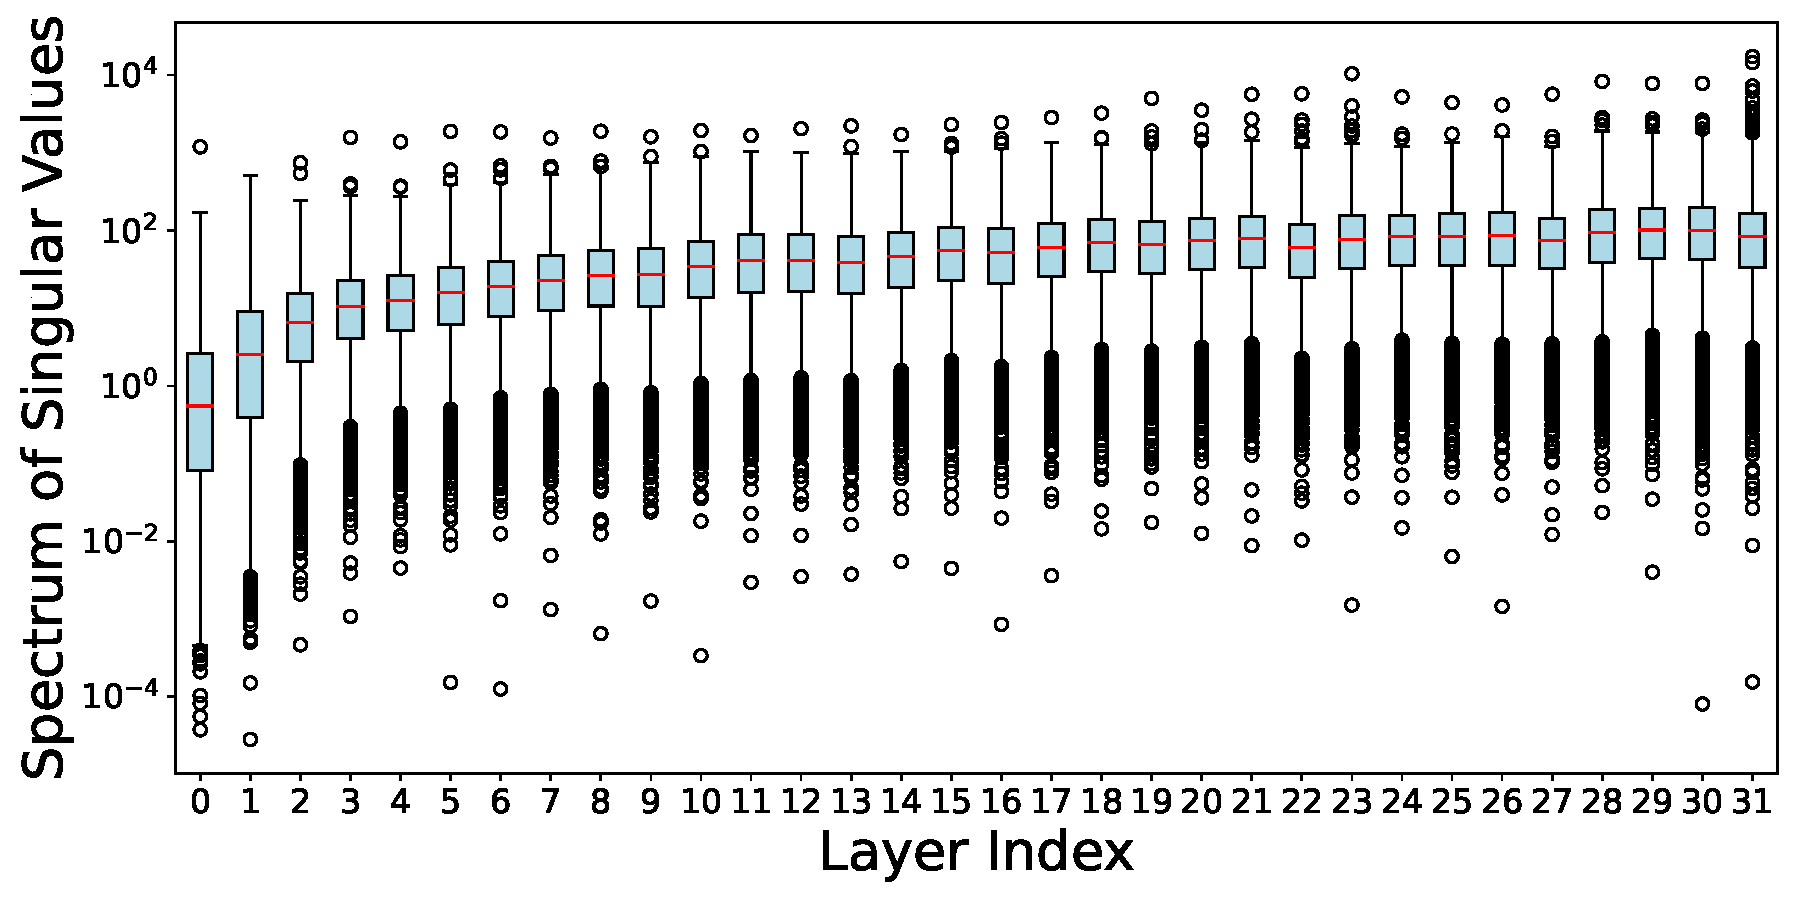
\includegraphics[width=1\textwidth]{Figures/q.pdf}
        \label{fig:q_spectrum}
    }
    \\
    \centering
    \subfigure[$W_K\times S_K$]{
        \includegraphics[width=1\textwidth]{Figures/K.pdf}
        \label{fig:v_spectrum}
    }
    \DeclareGraphicsExtensions.
    \caption{The singular value spectrum of the decomposed matrices across layers in LLaMA-7B.}
    \label{fig:spectrum_analysis}
\end{figure}

%\subsection{Implementation Details}
%\textbf{Implementation Details.} 
%\label{appendix:experimental_setup}
%To ensure a fair comparison, we followed ASVD~\citep{DBLP:journals/corr/abs-2312-05821} to randomly select 256 samples from WikiText-2 as the calibration data. 
%We followed the same configuration used in LLM-Pruner~\citep{DBLP:conf/nips/MaFW23} to use Alpaca~\citep{alpaca} dataset with 50K samples for parameter update in \sysname.
% All of our experiments are conducted on NVIDIA A100 GPUs.
%The inference efficiency experiment is conducted on both NVIDIA A100 GPU and AMD EPYC 7643 CPU while the other experiments are conducted on NVIDIA A100 GPUs.

\subsection{Spectrum Analysis of Singular Values decomposed by \sysname}
\label{appendix:spectrum_analysis}
In general, SVD is useful for compression when the matrix to be compressed shows a sharp decay of the singular values. Since \sysname decomposes the multiplication of the weight matrix $W$ and its corresponding whitening matrix $S$ instead of the original weight matrix $W$, which is different from the weight decomposition in the previous work~\citep{DBLP:journals/corr/abs-2312-05821,DBLP:conf/iclr/HsuHCLSJ22}, to study whether SVD compression is also applicable in \sysname, we select the Query ($W_Q$) and Key ($W_K$) weight matrices and show the spectrum of singular values of their multiplication with corresponding whitening matrices $S_Q$ and $S_K$. As shown in Figure~\ref{fig:spectrum_analysis}, most of the single values are less than or around 100 with only a few extremely large values, indicating that SVD is applicable in \sysname.


\subsection{Comparison with DRONE}
\label{appendix:comparison_with_drone}
\xin{
Previous work DRONE~\citep{DBLP:conf/nips/ChenYDH21} also proposes their data-aware method for SVD compression. They even provide a theoretical analysis to prove the optimal solution that their method achieves. Specifically, DRONE represents the low-rank compressed weight matrix $W'$ by $WM$. It performs SVD on both weight matrix $W = U_wS_wV_w^{T}$ and the transpose of input activation $X^T = U_xS_xV_x^{T}$ and then split these decomposed matrices as follows:}

$$
\begin{aligned}
& U_W=\left[\begin{array}{ll}
U_{W, r} & \bar{U}_{W, r}
\end{array}\right], S_W=\left[\begin{array}{cc}
S_{W, r} & 0 \\
0 & 0
\end{array}\right], V_W=\left[\begin{array}{ll}
V_{W, r} & \bar{V}_{W, r}
\end{array}\right] \\
& U_X=\left[\begin{array}{ll}
U_{X, t} & \bar{U}_{X, t}
\end{array}\right], S_X=\left[\begin{array}{cc}
S_{X, t} & 0 \\
0 & 0
\end{array}\right], V_X=\left[\begin{array}{ll}
V_{X, t} & \bar{V}_{X, t}
\end{array}\right] .
\end{aligned}
$$
\xin{
where $r$ and $k$ are the rank of the $W$ and $X$. $U_{W, r}, V_{W, r}, U_{X, t}, V_{X, t}$ denote corresponding row spaces and column spaces and $\bar{U}_{W, r}, \bar{V}_{W, r}, \bar{U}_{X, t}, \bar{V}_{X, t}$ are null spaces. Through theoretical deduction, DRONE converts the minimization of compression loss $||WX-W'X||_F = ||WX-WMX||_F$ to the minimization of $\left\|S_{W, r} V_{W, r}^T V_{X, t} S_{X, t}-S_{W, r} V_{W, r}^T M V_{X, t} S_{X, t}\right\|_F$, whose optimal value $L_{min}$ is the rank-k truncated SVD of $Z=S_{W, r} V_{W, r}^T V_{X, t} S_{X, t}$ by the fundamental property of SVD decomposition. To achieve the optimal value, DRONE formulates a solution $M = V_{W, r} S_{W, r}^{-1} Z_k S_{X, t}^{-1} V_{X, t}^T$, where $Z_k$ is the rank-k SVD truncation of $Z$. }

\xin{In short, compared with DRONE, \sysname is also optimal with the same theoretical compression loss as DRONE. Moreover, \sysname has \textbf{three} key advantages. Below is our detailed explanation.}


\xin{\textbf{\sysname is also optimal with the same theoretical compression loss as DRONE.}
% Although the motivation of \sysname originates from the SVD-based LLM compression methods, especially ASVD, and its motivation is to align the SVD truncation with the truncated singular values for a correct truncation, as discussed in Section 3.1, our theoretical analysis shows that \sysname is also optimal with the same compression loss as DRONE. 
The theoretical minimum compression loss $L_{min}$ is the F-norm loss of rank-k SVD truncation of $WX$, which has also been achieved by DRONE in their paper. Unlike DRONE, \sysname constructs the whitening matrix $S$ so that $S^{-1}X$ is orthonormal. Therefore, we have $||AS^{-1}X||_F = ||A||_F$. Suppose that we decompose $S$ with SVD to $U_s,S_s,V_s$, we can have $S_s = S_x$, $U_s = U_x, Us = Ux, V_s = QV_x$, where $Q$ is an orthogonal matrix. The matrix $WS$ to which \sysname applies SVD could be represented by $U_wS_wV_w^{T}U_sS_sV_s^{T}$. Suppose that we use $\boldsymbol{\operatorname{Trunc.}}(C)$ to represent the rank-k truncation of the matrix $C$ during SVD compression, the compression loss $L$ is derived as follows:}


\vspace{-5mm}
{\small
\begin{align*}
L &= ||WX-W'X||_F = ||(WSS^{-1}X -\boldsymbol{\operatorname{SVD}}(WS)S^{-1}X)||_F  = ||(WS -SVD(WS))S^{-1}X||_F\\
& = ||\boldsymbol{\operatorname{Trunc.}}(WS)S^{-1}X||_F = ||\boldsymbol{\operatorname{Trunc.}}(WS)||_F\\
&=||\boldsymbol{\operatorname{Trunc.}}(U_wS_wV_w^{T}U_sS_sV_s^{T})||_F =||\boldsymbol{\operatorname{Trunc.}}(WXQ^T)||_F = L_{min}
\end{align*}
}


\xin{Therefore, \sysname shares the same theoretical compression loss as DRONE. }



\xin{\textbf{Advantage \#1: DRONE incurs out-of-memory when compressing LLMs due to its requirement of storing the full large-scale activations, whereas \sysname is feasible.} To achieve data-awareness during compression, DRONE caches all input activations $X$ and spans them to calculate the corresponding singular vectors and singular values. In the DRONE paper, the authors apply DRONE to small LMs such as BERT. However, the activations generated by LLMs are often extremely large and are much larger than BERT. 
For example, to compress LLaMA-7B with 5,000 calibration data by DRONE, the total memory to cache the activation for a single weight matrix at a time is 5000 (data number) $\times$ 256 (seq\_len) $\times$ 11008 (dim) $\times$ 32 (fp32) $\div$ 1024 $\div$ 1024 $\div$ 1024 $=$ 419GB, which is more than 5 times larger than the memory provided by the NVIDIA A100 GPU, which has 80GB memory. Therefore, applying DRONE for LLM compression is infeasbile.  }

% \begin{wrapfigure}{r}{0.7\textwidth} % "r" 表示右侧，"0.5\textwidth" 控制宽度
%   \centering
%   \vspace{-5mm}
%   \dronelossTable
%   \vspace{-2mm}
% \end{wrapfigure}
\dronelossTable

\xin{In contrast, \sysname incrementally updates its $XX^T$ matrix by adding the $xx^T$ of each new input $x$. As such, \sysname eliminates the need to store the full activations, which requires only the storage of the matrix $XX^T$, which is considerably smaller than the full input activation. To compress LLaMA-7B with 5,000 calibration data, \sysname requires only 11008 $\times$ 11008 $\times$ 32 $\div$ 1024 $\div$ 1024 $\div$ 1024 $=$ 3.6GB. Compared to DRONE, \sysname achieves 116.38 times less memory reduction than DRONE. In our paper, we use WikiText-2 as a dataset. If we use DRONE, the total memory to cache the activation of a single weight matrix is larger than 24,600GB. In contrast, \sysname still requires 3.6GB of memory, which is more than 6,000 times less than DRONE. Due to this advantage, \sysname is much more practical to compress LLMs of size 7B or larger compared to DRONE.}

 \dronetimeTable
% \begin{wrapfigure}{r}{0.7\textwidth} % "r" 表示右侧，"0.5\textwidth" 控制宽度
%   \centering
%   \vspace{-5mm}
%   \dronetimeTable
% \end{wrapfigure}
\xin{\textbf{Advantage \#2: \sysname incurs much shorter compression time compared to DRONE.} DRONE involves more complex matrix operations, leading to longer compression time compared to \sysname. To illustrate this, we measured the time required by DRONE and \sysname to compress randomly generated weight and activation matrices of varying shapes under 50\% compression ratio. The results show that \sysname is approximately three times faster than DRONE.}

\xin{\textbf{Advantage \#3: \sysname has better numerical stability, which leads to superior empirical compression loss.}
 While \sysname shares the same theoretical compression loss as DRONE, DRONE’s higher complexity—stemming from additional SVD operations and inverse calculations on large-scale matrices—makes it less numerically stable compared to \sysname. This often results in higher empirical compression losses. To illustrate this, we compare \sysname and DRONE in terms of empirical compression losses for randomly generated matrices of various shapes. We also include the theoretical minimum value, represented by the rank-k Frobenius norm loss of $WX$. The results are summarized in the following table. As shown, we observe that \sysname achieves lower empirical compression losses than DRONE, underscoring its superior numerical stability.}



\flapTable

\subsection{Comparison with FLAP}
\label{appendix:flap_comparison}
\xin{
Recent work FLAP~\citep{DBLP:conf/aaai/AnZYTW24} is also a post-training structured-pruning method. Below we compare the perplexity of \sysname and FLAP on WikiText-2 under different compression ratios when compressing LLaMA-7B. As shown in~\cref{tab:flap}, \sysname consistently outperforms FLAP, especially under high compression ratios. }


\scalingTable

\subsection{Comparison with smaller LLMs pre-trained from scratch}
\label{appendix:pretrained_comparison}
To compare the performance between \sysname and scratch training, following the previous experimental design~\citep{DBLP:conf/nips/MaFW23}, we compress LLaMA-7B to the size of the 3B parameter with \sysname and select StableLM-3B~\citep{StableLM-3B-4E1T} as the baseline for comparison. As shown in Table~\ref{tab:scaling}. LLaMA-3B compressed from LLaMA-7B by \sysname achieves better accuracy in all datasets, indicating that \sysname could even achieve better accuracy than some scratch training methods. Furthermore, \sysname ensures higher throughput and lower memory consumption than StableLM-3B as shown in the table, which also meets our efficiency analysis and discussion in Section~\ref{subsec:inference_speedup}. 
% In the future, even though more and more smaller but more powerful LLMs will be obtained via scratch training, \sysname still holds its superiority from two aspects: (1) compressing more advanced larger LLMs to a smaller size with better accuracy. (2) Ensuring better inference efficiency with larger speedup and memory saving.


% \begin{wrapfigure}{r}{0.7\textwidth} % "r" 表示右侧，"0.5\textwidth" 控制宽度
%   \centering
%   \vspace{-5mm}
%   \timeTable
% \end{wrapfigure}

\timeTable

\subsection{Compression Speed Evaluation}
\label{appendix:compression_speed}
% \vspace{-2mm}
In addition to compression performance, we also evaluate the compression speed of \sysname and the baselines. Specifically, we measured the GPU hours used for \sysname and ASVD when compressing LLaMA-7B under 20\% compression ratio on an A100 GPU. The results are shown in~\cref{tab:time}. As shown, ASVD takes about $5.5$ hours, while \sysname completes the compression process in $3.5$ hours, which is $36\%$ times faster. When breaking down the time, most of the time consumed by ASVD is dedicated to searching for the specific compression ratio for each weight matrix based on its calculated importance score. In contrast, \sysname maintains a consistent compression ratio in all weight matrices and thus eliminates the time-consuming search process.

\subsection{Contents Generated from LLMs Compressed by \sysname and ASVD}
\label{sec:appendix_example}
Some examples of sentences generated by LLaMA-7B compressed with \sysname and ASVD are shown in~\cref{tab:visualization_lora}. 
%
The sentences generated by the model compressed by \sysname exhibit better fluency, relevance, and informativeness compared to those compressed by ASVD. More importantly, when the compression ratio is increased to 40\%, the previous state-of-the-art method ASVD completely loses its generation ability. 
In contrast, even when the compression ratio is up to 80\%, \sysname is still capable of generating complete sentences.
\exampleLoraTable




% \vspace{-3mm}


% \subsection{Comparison on extremely large-scale and more recent LLMs}
% \begin{wrapfigure}{r}{0.4\textwidth} % "r" 表示右侧，"0.5\textwidth" 控制宽度
%   \centering
%   \vspace{-4mm}
%   \morellmaccuracyTable
% \end{wrapfigure}

% \xin{
% To further show the generalization of \sysname, we compare its performance with other SVD-based baselines on extremely large-scale and more recent LLMs. Below shows the perplexity of \sysname and other baselines on WikiText-2 when compressing LLaMA-2 70B~\citep{DBLP:journals/corr/abs-2307-09288} and LLaMA-3 8B~\citep{DBLP:journals/corr/abs-2407-21783} under 20\% compression ratio. For LLaMA-2 70B, we only apply truncation-aware data whitening of \sysname without parameter update with sequential low-rank approximation due to the limited computational budget. OOM means that running the algorithm causes out-of-memory on 4 A100 GPUs. As shown, \sysname still consistently outperforms other baselines when applied on these two LLMs.}





\subsection{More Ablation Studies}
\label{appendix:more_ablation}
\xin{
\textbf{\sysname + Normal LoRA Fine-tuning v.s. \sysname + Sequential LoRA fine-tuning.} To illustrate the superiority of the designed parameter update with the sequential low-rank approximation in \sysname, which is a kind of sequential LoRA fine-tuning strategy over the normal LoRA fine-tuning strategy, we compare the compression performance of \sysname by applying either of these two fine-tuning strategies. Let's denote \sysname (SFT) as \sysname by applying sequential LoRA fine-tuning and \sysname (NFT) as \sysname by applying normal LoRA fine-tuning. As shown in~\cref{tab:lora_add}, \sysname (SFT) consistently outperforms \sysname (NFT), which also reaffirms our analysis in~\cref{subsec:lora_finetunig} that optimizing both low-rank matrices $W_u, W_v$ at the same time is not stable and may lead to poor fine-tuning performance.}

\loraaddTable

\xin{
\textbf{ASVD + Sequential LoRA Fine-tuning v.s. \sysname + Sequential LoRA Fine-tuning.} Although the designed sequential LoRA fine-tuning strategy could also be applied in other SVD-based LLM compression methods, other methods' performance is still poorer than \sysname even when integrated with this strategy for enhancement. To illustrate this, we compare the performance of the previous state-of-the-art method ASVD when applied with the sequential LoRA finetuning with \sysname. Let's denote \sysname (SFT) as \sysname by applying sequential LoRA fine-tuning and ASVD (SFT) as ASVD by applying sequential LoRA fine-tuning. As shown in~\cref{tab:lora_add}, \sysname (SFT) consistently outperforms ASVD (SFT) under various compression ratios.}

% \begin{wrapfigure}{r}{0.4\textwidth} % "r" 表示右侧，"0.5\textwidth" 控制宽度
%   \centering
%   \vspace{-3mm}
%   \orthoTable
% \end{wrapfigure}
% \xin{
% \textbf{Orthogonality of whitening matrix on inference activations.} 
% Below we randomly select three weight matrices $W_1,W_2,W_3$ in LLaMA-7B and compute their on-the-fly whitening matrix $S_{fly}$ computed during inference. To test whether $S_{pre}$ precomputed on the calibration data can also make the inference activation orthogonal like $S_{fly}$, we measure the difference between $S_{fly}S_{fly}^T$ and $S_{pre}S_{pre}^T$ in the MSE format, e.i., $\frac{1}{N}||S _{fly} S _{fly}^T-S _{pre} S _{pre}^T||_F^2$, where $N$ is the number of elements in $S _{pre}S _{pre}^T$. As shown in~\cref{tab:orthogonality}, the difference is small, indicating that the pre-computed whitening matrix $S _{pre}$ is still effective in making the inference activation orthogonal to ensure the alignment between SVD truncation and compression loss.}

\subsection{Limitations}
There are three limitations of \sysname, which are left for future work.

\textbf{(1) The compression accuracy still needs to be improved under the high compression ratio.}
Although \sysname has achieved the state-of-the-art performance compared to previous works such as FWSVD and ASVD, its compression accuracy still suffers from degradation, especially under the high compression ratio. To enhance the practicability of \sysname in real-world scenario, its accuracy should be at least comparable to that of the quantization method, including both low-bit and high-bit quantization, rather than being combined with the quantization methods for usage.

\textbf{(2) The latency of \sysname needs to be optimized while being used to compress the KV cache.} As discussed in~\cref{subsec:inference_speedup}, \sysname can also be applied to compress the KV cache for memory saving during inference. However, this benefit does not come free. In fact, due to the additional calculation caused by recovering the original key and value states, the inference speed will be impacted by compressing the KV cache with \sysname, which should be optimized in the future.


\textbf{(3) \sysname should be better guided for high-quality generation.} Although \sysname achieves low perplexity, as demonstrated in~\cref{tab:dataset_acc}, it is still possible to generate low-quality content, such as repeated words even under low compression ratios. This phenomenon of compressed LLM has also been mentioned in previous work~\citep{DBLP:conf/nips/MaFW23} and should be eliminated in the future by guiding the compressed LLM for outputting high-quality generation.